\documentclass[12pt,a4paper]{article}
% 如果需要中文支持，推荐使用xeCJK + 字体设置
% \usepackage{xeCJK}
% \setCJKmainfont{SimSun}  % 示例：宋体，可根据系统字体情况更换
\usepackage{ctex}
\setlength{\parindent}{2em}
\setlength{\parskip}{0pt} % 确保段落之间没有额外的空行间距


\usepackage{amsmath}      % 数学公式（如有需要）
\usepackage{graphicx}     % 插图
\usepackage{geometry}     % 调整页边距
\usepackage{fancyhdr}     % 自定义页眉页脚
\usepackage{indentfirst}  % 中文首行缩进
\usepackage{calc}         % 允许做长度运算(测量文字宽度等)
\usepackage{titlesec}
\usepackage{booktabs} % 解决 \midrule 和 \bottomrule 报错
\usepackage{enumitem} % 支持自定义列表格式
\usepackage{float}    % 支持强制浮动位置
\usepackage{siunitx}

% 设置 \section 级标题为：加粗、大字号（如 \Large）
\titleformat{\section}
	{\bfseries\large}    % 标题自身的格式
	{\thesection}        % 标题编号的显示方式
	{1em}                % 编号与标题文字之间的间距
	{}                   % 在标题文字前后可插入额外代码，此处为空
	
% 设置 \subsection 级标题为：加粗、中等字号（如 \normalsize）
\titleformat{\subsection}
	{\bfseries\normalsize}
	{\thesubsection}
	{1em}
{}

% 页面设置（可根据需要微调）
\geometry{
	left=2cm,
	right=2cm,
	top=1cm,
	bottom=1.5cm
}

% 不需要过大的行距，使用较接近单倍行距的设置
\renewcommand{\baselinestretch}{1.2}

% 仅在页脚居中显示页码，页眉保持为空
\pagestyle{fancy}
\fancyhf{}  % 清空默认的页眉页脚
\fancyfoot[C]{\thepage}
\renewcommand{\headrulewidth}{0pt}
\renewcommand{\footrulewidth}{0pt}

% 首行缩进2字符(中文习惯)
\setlength{\parindent}{0pt}
\setlength{\leftskip}{2em}

\begin{document}
	%-------------------------------------------------------
	% 1 并排两个minipage：左标题、右校徽
	%   - 0.65\textwidth + 0.35\textwidth = \textwidth
	%   - 如果校徽过大或过小，可改宽度，如 0.25\textwidth、0.3\textwidth 等
	%   - 如果想让标题更大，可将 \Huge 改成 \huge 或 \LARGE
	%-------------------------------------------------------
	\noindent
	\hspace{-2em}
	\begin{minipage}[c]{0.65\textwidth}
		\raggedright
		{\fontsize{40pt}{60pt}\selectfont 物理实验报告}
	\end{minipage}
	\begin{minipage}[c]{0.35\textwidth}
		\raggedleft
		% 强制把校徽拉大到 0.35\textwidth 宽度 (高度自动匹配)
		% 若想指定高度,可用 "height=3cm" 等. 二选一即可.
		
\includegraphics[width=\linewidth, trim={20cm 20cm 20cm 20cm}, clip]{university_logo.png}
	\end{minipage}

	\vspace{-1em}
	

	%下方画两条分割线，并在两线之间写学号、姓名、日期、时间
	
	\hrule
	\vspace{0.6em}
	\noindent
	\begin{tabular}{l l l l}
    学号：12411434 & 姓名：{郑宇轩} &
    日期：2025.09.26 & 时间：周五下午
	\end{tabular}
	\vspace{0.4em}
	\par
	\hrule

	
	\section*{\textbf{一. 实验名称：声速的测量}}
	
	\section*{\textbf{二. 实验目的}}
	\begin{enumerate}
		\item 了解压电换能器的工作原理。
		\item 学习超声波的产生、发射和接收方法。
		\item 掌握驻波法和相位法测量波长和声速的方法。
	\end{enumerate}

	\section*{\textbf{{三. 实验原理}}}
	
	% \begin{enumerate}
		声速测量的常用方法有两类, 一类测量声波传播距离 $L$ 和时间间隔 $t$, 即可根据
$$v=\frac{L}{t}$$
计算出声速; 另一类是测出频率 $f$ 和波长 $\lambda$, 利用关系式
\begin{equation} \label{eq:v_lambda_f}
v=f\cdot\lambda
\end{equation}

声波在空气中的传播速度与声波的频率无关, 而只取决于空气本身的性质。声速的理论值由下式决定:
\begin{equation} \label{eq:v_theory}
v=\sqrt{\frac{\gamma RT}{\mu}}
\end{equation}
式中, $\gamma$ 为空气定压比热容与定体比热容之比, $R$ 为普适气体常量, $\mu$ 为气体的摩尔质量, $T$ 为热力学温度。在 $0^{\circ}C$ 时, 声速 $v_{0}=331.45m/s$。显然在 $t^{\circ}C$ 时的声速应为:
\begin{equation} \label{eq:v_temp}
v_{t}=v_{0}\sqrt{\frac{T}{273.15}}=v_{0}\sqrt{1+\frac{t}{273.15}}
\end{equation}
如果测到了声速, 由 \eqref{eq:v_theory} 式还可求出空气的比热容比。

实验中超声波是由交流电信号产生的, 所以 \eqref{eq:v_lambda_f} 式中声波的频率 $f$ 就是交流电信号的频率, 由信号发生器中的频率显示可直接读出。因此, 本实验的主要任务就是测量声波的波长。

测量声波波长方法有驻波法、相位法两种。

\subsection*{1. 驻波法}
\begin{figure}[h]
    \centering
    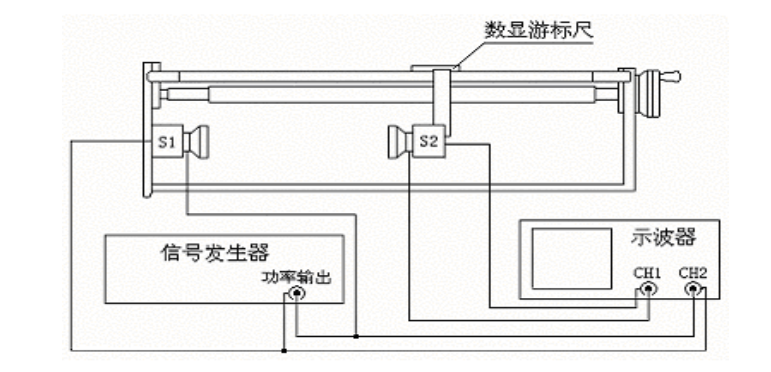
\includegraphics[width=0.9\textwidth]{1.png} % 占位符：请替换为实际的实验装置图
    \caption{实验装置图}
    \label{fig:1}
\end{figure}
实验装置如图 1 所示, 超声发射器 $S_{1}$ 作为超声波源。信号发生器发出的信号接入 $S_{1}$ 后, $S_{1}$ 即发射出一平面超声波。超声波接收器 $S_{2}$, 接收一部分超声波转换成电信号后, 输入示波器进行观察, 同时反射一部分超声波。这样, 由 $S_{1}$ 发出的超声波和由 $S_{2}$ 反射的超声波在 $S_{1}$、$S_{2}$ 之间叠加相干而出现驻波。

设声源在坐标轴原点, 由声源发出的平面简谐波沿 $x$ 轴正向传播, 为入射波, 经一个理想平面反射后沿 $x$ 轴负方向传播, 为反射波。
入射波方程为:
\begin{equation} \label{eq:incident}
x_{1}=A\cos 2\pi\left(ft-\frac{x}{\lambda}\right)
\end{equation}
反射波方程为:
\begin{equation} \label{eq:reflected}
x_{2}=A\cos 2\pi\left(ft+\frac{x}{\lambda}\right)
\end{equation}
在两波相遇处, 合成的声波为:
\begin{equation} \label{eq:standing_wave}
x=\left(2A\cos 2\pi\frac{x}{\lambda}\right)\cos 2\pi ft
\end{equation}
上式表明, 两波合成的结果是驻波。在两波相遇处各点都在作同频率的振动, 而各点的振幅 $\left(2A\cos 2\pi\frac{x}{\lambda}\right)$ 是位置的余弦函数。对应于 $\left|\cos 2\pi\frac{x}{\lambda}\right|=1$, 即 $x=\pm K\frac{\lambda}{2}(K=0,1,2,\cdots)$ 处, 振幅最大为 $2A$, 称为波腹; 对应 $\left|\cos 2\pi\frac{x}{\lambda}\right|=0$, 即 $x=\pm(2K+1)\frac{\lambda}{4}(K=0,1,2,3,\cdots)$ 处, 振幅最小为零, 称为波节。其余各点的振幅在 $0$ 和最大值之间, 两相邻波腹 (或波节) 间的距离均为 $\frac{\lambda}{2}$。

当移动 $S_{2}$, 使 $S_{1}$ 与 $S_{2}$ 之间的距离为半波长的整数倍时, 即
\begin{equation} \label{eq:驻波条件}
l=n\frac{\lambda}{2}(n=1,2,3\cdots)
\end{equation}
示波器上可观察到信号幅度的极大值 (或极小值)。相邻两极值点之间的距离为 $\frac{\lambda}{2}$。

\subsection*{2. 相位比较法}
从发射器 $S_{1}$ 发出的超声波近似于平面波, 沿着此波传播方向上, 相位相同或相位差为 $2\pi$ 的整数倍的任意两点位置之间的距离等于波长的整数倍, 即 $l=n\lambda$ ($n$ 为正整数)。当接收器端面垂直于波的传播方向时, 其端面上各点都具有相同的位相。沿传播方向移动接收器 $S_{2}$ 时, 总可找到一个位置使得接收到的信号与激励信号即函数信号发生器发出的信号同相。继续移动 $S_{2}$, 直到接收到的信号再一次和激励信号同相时, 移过的这段距离必然等于超声波的波长。

相位差可根据两个互相垂直的简谐振动的合成所得到的李萨如图来测定。将信号发生器发出的信号接入示波器的通道1 (CH1) 输入端, 将 $S_{2}$ 接收到的电信号接到示波器的通道2 (CH2) 输入端, 并使两路信号叠加一起, 由于两端电信号频率相同, 因而叠加合成如下图的李萨如图形, 图的形状由两信号的相位差 $\Phi$ 决定。假如初始时图形如图 \ref{fig:lissajous} (a), $S_{2}$ 移动距离为半波长时, 图形变化为图 \ref{fig:lissajous} (e); $S_{2}$ 移动距离为 $\lambda$ 时, 图形变回图 \ref{fig:lissajous} (a), 所以通过对李萨如图形的观测, 就能确定声波的波长。

\begin{figure}[h]
    \centering
    % 使用一个占位符来表示李萨如图形，原图中 a-e 分别对应 Phi=0, pi/4, pi/2, 3pi/4, pi
    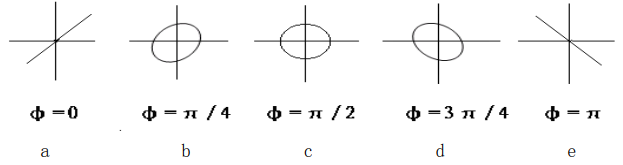
\includegraphics[width=0.8\textwidth]{2.png} % 占位符：请替换为实际的李萨如图形
    \caption{同频率互相垂直的谐振动合成的李萨如图形}
    \label{fig:lissajous}
\end{figure}
	
	\section*{\textbf{{四. 实验仪器}}}
	信号发生器，示波器，超声声速测定仪等。

	\section*{\textbf{{五. 实验内容}}}

	\begin{enumerate}
		\item 调整仪器使系统处于最佳工作状态
		
		\begin{enumerate}
			\item 实验装置和接线如图 1 所示。调节发射换能器的端面 $S_{1}$, 使其与游标卡尺滑动方向垂直; 接收换能器 $S_{2}$ 的端面与 $S_{1}$ 平行。
			\item 寻找系统的谐振频率, 并调整低频信号发生器, 使其输出频率为系统的谐振频率。具体方法是: 旋转右侧手轮, 移动游标和接收换能器 $S_{2}$, 使 $S_{1}$ 和 $S_{2}$ 端面距离 $5cm$ 左右, 调整低频信号发生器的输出强度和接收增益, 同时调整示波器, 使示波器屏幕上有适当的信号幅度; 然后旋转手轮移动游标和 $S_{2}$, 找到信号最强的位置, 再调节信号发生器的输出频率, 使示波器上的信号幅度最大。此时, 信号发生器的输出频率即为本系统的谐振频率。上述过程反复数次, 以寻找本系统准确的谐振频率 $f_{0}$。
		\end{enumerate}

		\item 驻波法测量波长和声速
		
			\begin{enumerate}
				\item 调整信号发生器输出频率为本系统准确的谐振频率，即令$f = f_{0}$。
				\item 测量前旋转手轮, 将 $S_{2}$ 从一端缓慢移向另一端, 并来回几次, 观察示波器上信号幅度的变化, 了解波的干涉现象。测量时, 选择一个信号幅度最大处为起点, 记下 $S_{2}$ 的位置, 缓慢移动 $S_{2}$, 增大 (或减小) $S_{1}$ 与 $S_{2}$ 的间距, 依次记录每次信号幅度最大时 $S_{2}$ 的位置 $X_{1}, X_{2}, X_{3}, \cdots, X_{n}$ 共 $12$ 个值。
				\item 用逐差法处理数据, 求出超声波的波长, 再用公式 $v=f\times\lambda$, 计算声速。
			\end{enumerate}

		\item 相位比较法测量波长和声速
		
			\begin{enumerate}
				\item 调整信号发生器输出频率为本系统准确的谐振频率 $f_{0}$。增加一根导线, 把信号发生器的输出信号直接接入示波器的 $X$ 输入端 (CH1 通道), 调节示波器使屏上出现李萨如图形。
				\item 缓慢移动 $S_{2}$, 增大 (或减小) $S_{1}$ 与 $S_{2}$ 的间距, 示波器上就会反复出现周期性的李萨如图形。选择李萨如图形为直线时为起点, $S_{2}$ 每移动整个波长, 就会出现一次直线图形。依次记录示波器上出现\textbf{与初始直线处于相同象限}的直线时 $S_{2}$ 所对应的位置 $X_{1}, X_{2}, X_{3}, \cdots, X_{n}$ 共 $12$ 个值。
				\item 用逐差法处理数据, 求出超声波的波长, 再用公式 $v=f\times\lambda$, 计算声速。
			\end{enumerate}

		\item 计算使用驻波法时的不确定度。
		
	\end{enumerate}
	
	\section*{\textbf{{六. 数据记录}}}
	
	原始测量数据见附表 1。

	\section*{\textbf{{七. 数据处理}}}

	\subsection*{1. 驻波法}
\begin{enumerate}
    \item \textbf{计算声速}
    
	声波频率 $f = f_{0} = 35.6$kHz。

	实验温度 $T = 25.5^{\circ}\mathrm{C}$

	测得波长：
    
	\begin{footnotesize}
	$$\lambda_{1}=\frac{(X_{7}-X_{1})+(X_{8}-X_{2})+(X_{9}-X_{3})+(X_{10}-X_{4})+(X_{11}-X_{5})+(X_{12}-X_{6})}{6\times3}$$

	$$=\frac{86.760-57.130+91.639-61.977+96.668-66.935+101.499-71.730+106.450-76.940+111.510-81.836}{6\times3}$$

		$$=9.888\mathrm{mm}$$

	\end{footnotesize}

	测得声速：

    $$v_{1}=\lambda_{1}\times f_{0}=9.888\times 10^{-3} \times 35.6\times 10^{3} = 352.01\mathrm{m/s}$$

    由参考声速 
	$$v_{t}=v_{0}\sqrt{\frac{T_{t}}{T_{0}}}=v_{0}\sqrt{1+\frac{T}{273.15}}=331.45\sqrt{1+\frac{25.5}{273.15}}=346.58m/s$$

    则相对误差 $\epsilon_{1}=\left|\frac{352.01-346.58}{346.58}\right|\times 100\%=1.57\%$

    \item \textbf{不确定度计算}
    
    \textbf{波长不确定度}

    \begin{enumerate}
        \item[1)] A 类不确定度
        $$u_{A}(\lambda)=\sqrt{\frac{\sum_{i=1}^{n}(\Delta X_{i}-\overline{\Delta X})^{2}}{n(n-1)}}$$
        $$u_{A}(\lambda)=\sqrt{\frac{(29.63-29.663)^{2}+\cdots+(29.674-29.663)^{2}}{5\times 6}}=0.2313mm$$


        \item[2)] B 类标准不确定度
		
		仪器最大允差 $\Delta_{B} = 0.01$mm
		取置信系数 $C = 3$

		$$u_{B}(\lambda)=\frac{\Delta_{B}}{C}=\frac{0.01}{3}=0.0033mm$$
        
    	\item[3)]合成不确定度
		
		$P=0.95$时, $n=6$的 $t$因子 $t_{0.95} = 2.57$；$k_{p} = 1.96$。

		$$u_{0.95}(\lambda)=\sqrt{(t_{0.95}u_{A}(\lambda))^{2}+(k_{p}u_{B}(\lambda))^{2}}=\sqrt{(2.57\times 0.2313)^{2}+(1.96\times 0.0033)^{2}}=0.594mm$$
    \end{enumerate}

    \textbf{谐振频率不确定度}
	
	$$u_{B}(f)=\frac{\Delta_{B}}{\sqrt{3}}=\frac{0.001kHz}{\sqrt{3}}=0.577Hz$$

    $u_{f}=k_{p}\times u_{B}(f)=1.96\times 0.577=1.13Hz$

    \textbf{不确定度的传递}

	 由 $v=f\cdot\lambda$ 可得
    $$\frac{u_{0.95}(v)}{v}=\sqrt{\left(\frac{u_{\lambda}}{\lambda}\right)^{2}+\left(\frac{u_{f}}{f}\right)^{2}}=\sqrt{\left(\frac{0.594}{9.888}\right)^{2}+\left(\frac{1.13}{35600}\right)^{2}}=0.0601$$
    故 $u_{0.95}(v)=0.0601\times 352.01 = 21.146\mathrm{m/s}\quad P=0.95$.

    则驻波法测得声速：
	
	$$v_1 = (352.01\pm 21.91)\mathrm{m/s} \quad P = 0.95$$

\end{enumerate}

\subsection*{2. 相位比较法}


	声波频率 $f = f_{0} = 35.6$kHz。

	实验温度 $T = 25.5^{\circ}\mathrm{C}$

	测得波长：
    
	\begin{footnotesize}
	$$\lambda_{2}=\frac{(X_{7}-X_{1})+(X_{8}-X_{2})+(X_{9}-X_{3})+(X_{10}-X_{4})+(X_{11}-X_{5})+(X_{12}-X_{6})}{6\times6}$$

	$$=\frac{115.700-57.006+125.539-66.791+135.328-76.351+145.140-86.110+154.920-96.059+164.569-105.983}{6\times6}$$

		$$=9.803\mathrm{mm}$$

	\end{footnotesize}

	测得声速：

    $$v_{2}=\lambda_{2}\times f_{0}=9.803\times 10^{-3} \times 35.6\times 10^{3} = 348.99\mathrm{m/s}$$

    由参考声速 
	$$v_{t}=v_{0}\sqrt{\frac{T_{t}}{T_{0}}}=v_{0}\sqrt{1+\frac{T}{273.15}}=331.45\sqrt{1+\frac{25.5}{273.15}}=346.58m/s$$

    则相对误差 $\epsilon_{2}=\left|\frac{348.99-346.58}{346.58}\right|\times 100\%=0.696\%$


	\section*{\textbf{{九. 问题思考}}}

	\begin{enumerate}
		\item \textbf{固定两换能器的距离改变频率，以求声速，是否可行？}

		理论成立, 实际操作不可行。首先, 改变的频率较低时, 声波波长较大, 所需实验器材较长, 不合实际。同时, 在较低频率时易受其他声波干扰导致误差较大。其次, 改变的频率过高, 使声波波长较小, 易导致测量误差增加使结果误差增大。所以不可行。
		
		\item \textbf{各种气体中的声速是否相同，为什么？}
		
		由声速的理论值由公式
    $$v=\sqrt{\frac{\gamma RT}{\mu}}$$
    可得, 不同气体, 空气定压比热容与定体比热容之比 $\gamma$ 以及气体的摩尔质量 $\mu$ 均不同, 因此同一温度不同气体中的声速不同。
	\end{enumerate}

	
	\section*{\textbf{{十. 实验结论}}}
	
	本实验在室温为 $25.5^{\circ}$C 时:
\begin{enumerate}
    \item 使用驻波法测量得到声速为 $v_1 = (352.01\pm 21.91)\mathrm{m/s} \quad P = 0.95$，相对误差为 $1.57\% $。
    \item 使用相位比较法测量得到声速为 $v=348.99/s$, 相对误差为 $0.696\% $
\end{enumerate}
	
	

\end{document}